\documentclass[12pt,notitlepage]{article}
%\usepackage{jmlda}
\usepackage[T2A]{fontenc}
\usepackage[utf8]{inputenc}
\usepackage{amsmath,amssymb,mathrsfs,mathtext}
\usepackage[russian]{babel}
\usepackage{graphicx}
\usepackage{enumerate}
\usepackage{fancyhdr}
\usepackage{cite}
%\usepackage[margin=0.75in]{geometry}
\usepackage{a4wide}
\input xy
\xyoption{all}

\usepackage{dcolumn}
\usepackage{caption} % ïîäïèñè ê ðèñóíêàì â ðóññêîé òèïîãðàôñêîé òðàäèöèè
\DeclareCaptionFormat{GOSTtable}{#1~#3}
\DeclareCaptionLabelSeparator{fill}{\hfill}
\DeclareCaptionLabelFormat{fullparents}{\bothIfFirst{#1}{~}}
\captionsetup[table]{
  format=GOSTtable,
  labelfont=bf,
  labelformat=fullparents,
  labelsep=fill,
  justification=centering,
  singlelinecheck=false
  }
\DeclareCaptionFormat{GOSTfigure}{#2#1~#3}
\DeclareCaptionLabelSeparator{fill}{\hfill}
\DeclareCaptionLabelFormat{fullparents}{\bothIfFirst{#1}{~}#2}
\captionsetup[figure]{
  format=GOSTtable,
  labelfont=bf,
  labelformat=fullparents,
  labelsep=fill,
  justification=centering,
  singlelinecheck=false
  }

\pagestyle{fancy}
\fancyhead{}
\renewcommand{\headrulewidth}{0pt}
\DeclareMathOperator*{\argmin}{arg\,min}
\DeclareMathOperator*{\argmax}{arg\,max}
\begin{document}
%\renewcommand{\baselinestretch}{1. 5}
\title{Глубокое обучение с использованием графического процессора NVIDIA и облачного сервиса AWS: методические рекомендации\thanks{Работа выполнена при поддержке РФФИ (проект 16-37-00488)}}
%\begin{center}
%\end{center}
 %[О.\,Ю.~Бахтеев, М.\,С.~Попова] % список авторов, выводимый в заголовок; не нужен, если он не отличается от
	
%\email
% {bakhteev@phystech.edu, maria$\_$popova@phystech.edu, strijov@ccas.ru}
%\organization
% {$^1$Московский физико-технический институт; $^2$Вычислительный центр РАН}


\maketitle

\author 
  % список авторов для колонтитула; не нужен, если основной список влезает в колонтитул
 {О.\,Ю.~Бахтеев\footnote{Московский физико-технический институт, bakhteev@phystech.edu}, М.\,С.~Попова\footnote{Московский физико-технический институт, maria\_popova@phystech.edu}, В.\,В.~Стрижов\footnote{Вычислительный центр им. А.~А. Дородницына Федерального исследовательского центра <<Информатика и управление>> Российской академии наук, strijov@ccas.ru}} % основной список авторов, выводимый в оглавление

\abstract{
\emph{Аннотация}. Работа посвящена построению сети глубокого обучения и оптимизации ее параметров с помощью вычислительных мощностей графического ускорителя на основе сервиса облачных вычислений Amazon Web Services. Рассматривается задача классификации временных рядов. Для ее решения строится сеть глубокого обучения: суперпозиция универсальных моделей. В качестве исследуемой структуры сети рассматривается композиция ограниченной машины Больцмана, автокодировщика и двухслойной нейросети. Анализируется зависимость ошибки классификации от числа параметров и размера обучающей выборки. В качестве иллюстрирующего примера рассматривается задача классификации временных рядов акселерометра мобильного телефона. Приведены рекомендации по использованию програмного обеспечения, предназначенного для решения задач глубокого обучения. 

\emph{Abstract}. The paper provides a guidance on deep learning net construction and optimization using GPU. The paper proposes to use GPU-instances on the cloud platform Amazon Web Services. The problem of time series classification is considered. The paper proposes to use a deep learning net, i.e. a multilevel superposition of models, belonging to the following classes: Restricted Boltzman Machines, autoencoders and neural nets with softmax-function in output. The proposed method was tested on a dataset containing time segments from mobile phone accelerometer. The analysis of relation between classification error, dataset size and superposition parameter amount is conducted. 

\emph{Keywords}:
 классификация временных рядов, глубокое обучение, суперпозиция моделей, автокодировщик, ограниченная машина Больцмана, Theano, Amazon Web Services, Autoencoder, CUDA.
}




\section{Введение}
В данной работе рассматривается задача построения сети глубокого обучения с использованием средств библиотеки NVIDIA CUDA и сервиса облачных вычислений Amazon Web Services (далее --- AWS). Решается задача классификации временных рядов, где
под временным рядом понимается упорядоченный по времени набор изменения некоторой случайной величины. Для решения этой задачи используются методы глубокого обучения. Под глубоким обучением понимается область машинного обучения, посвященная построению нелинейных моделей классификации или регрессии, элементы суперпозиции которых описывают соответствующий уровень признакового агрегирования данных~\cite{foundamentals}.

Решению прикладных задач методами глубокого обучения посвящено значительное число современных работ. Работы~\cite{ts1,ts2,ts3} посвящены классификации временных рядов с использованием методов глубокого обучения. В работе~\cite{ts2} используются рекуррентные нейронные сети, т.~е. сети, содержащие циклические связи~\cite{foundamentals}. В работе~\cite{ts3} для классификации временных рядов рассматриваются различные комбинации ограниченной машины Больцмана, автокодировщика и двухслойной нейронной сети. Исследуется суперпозиция, состоящая из ограниченной машины Больцмана, автокодировщика и двухслойной нейронной сети~\cite{foundamentals}. Работы~\cite{reg1,reg2,reg3,reg4} посвящены регуляризации сетей глубокого обучения. В работах~\cite{stab1,stab2} рассматривается проблема неустойчивости сети. В работе~\cite{stab1} исследуется поведение модели глубокого обучения как липшицевой функции. Работы~\cite{speed1,speed2,speed3} посвящены ускорению процесса решения оптимизационных задач, возникающих при работе с сетями глубокого обучения. Работы~\cite{stab2, ada} посвящены построению адаптивных моделей глубокого обучения. Работа~\cite{recrbm} посвящена рекуррентной модификации модели ограниченной машины Больцмана~\cite{rbm} для классификации временных рядов. Схожие идеи предлагаются в работе~\cite{rae}, посвященной построению рекурсивного автокодировщика. В работе~\cite{sparse} рассматривается регуляризация автокодировщика, позволяющая регулировать разреженность внутреннего слоя автокодировщика. В работе~\cite{denoise} рассматривается принцип работы варианта автокодировщика, задачей которой является фильтрация шума входного сигнала.

В данной статье решается прикладная задача классификации временных рядов. В качестве данных для вычислительного эксперимента используются данные с акселерометров мобильных телефонов~\cite{wisdm}. Эксперимент проводится с использованием Theano~\cite{theano1, theano2} --- библиотеки для вычислений для языка Python. Theano активно используется для построения моделей глубокого обучения, а также для построения более специализированных библиотек~\cite{lasagne, pylearn}. Функции вычислений Theano компилируются, что позволяет выполнять вычисления за приемлемое время. Другой отличительной особенностью Theano является возможность применения графического процессора с использованием архитектуры параллельных вычислений CUDA~\cite{cuda}. Также в экспериментальном режиме доступна возможность применить интерфейс OpenCL~\cite{cl}, что позволяет использовать для обучения нейросетей графические процессоры не только NVIDIA, но и других производителей, например Xilinx. В данной работе описывается эксперимент, направленный на сравнение эффективности обучения искусственных нейронных сетей на центральном процессоре и на графическом процессоре компьютера. Приводятся рекомендации по технической реализации классификации с использованием средств сервиса облачных вычислений AWS. Для решения задачи оптимизации используется алгоритм обратного распространения ошибок с послойным предобучением сети и дальнейшей настройкой параметров всех слоев~\cite{fine}.
В качестве альтернативного инструмента для решения задачи с использованием глубокого обучения рассматривается программное обеспечение для решения задач классификации временных рядов на языке Matlab.

\section{Формальная постановка задачи}
Пусть задана выборка \begin{equation}\label{eq:dataset}\mathfrak{D} = \{(\mathbf{x}_i,y_i)\}, i = 1,\dots,N,\end{equation} состоящая из множества пар <<объект - класс>>, $\mathbf{x}_i \in \mathbb{R}^n$. Каждый объект $\mathbf{x}$ принадлежит одному из $Z$ классов с меткой $y_i \in \mathbf{Y} = \{1,\dots,Z\}$.

Моделью классификации или сетью глубокого обучения $\mathbf{f}$ назовем суперпозицию функций
\begin{equation}
\label{eq:main}
 \mathbf{f}(\mathbf{w}, \mathbf{x}) = \boldsymbol{{\mu}}_1(\boldsymbol{\mu}_2(\dots \boldsymbol{\mu}_K(\mathbf{x}))): \mathbb{R}^n \to [0,1]^Z,
\end{equation}
где $\boldsymbol{\mu}_k, k \in \{1,\dots,K\}$, --- модели, параметрическое семейство вектор-функции; $\mathbf{w}$ --- вектор параметров моделей;
$r$-ю компоненту вектора $\mathbf{f}(\mathbf{x},\mathbf{w})$ будем интерпретировать как вероятность отнесения объекта $\mathbf{x}_i$ к классу с меткой $r$.

Требуется минимизировать функцию ошибки $S$ на обучающей выборке $\mathfrak{D}$,
где $S$ --- сумма отрицательных логарифмов правдоподобия~\cite{nnl} по всем объектам выборки:
\[
 \hat{\mathbf{w}} = \argmin_\mathbf{w} S(\mathbf{w}|\mathfrak{D}),
\]
где
\[
 S(\mathbf{w}|\mathfrak{D}) = -\sum_{(\mathbf{x},y) \in \mathfrak{D} } \sum_{r=1}^Z [y_i = r] \text{log} p(y=r|\mathbf{x},\mathbf{w}).
\]

\begin{figure}[h!]
 \centering
  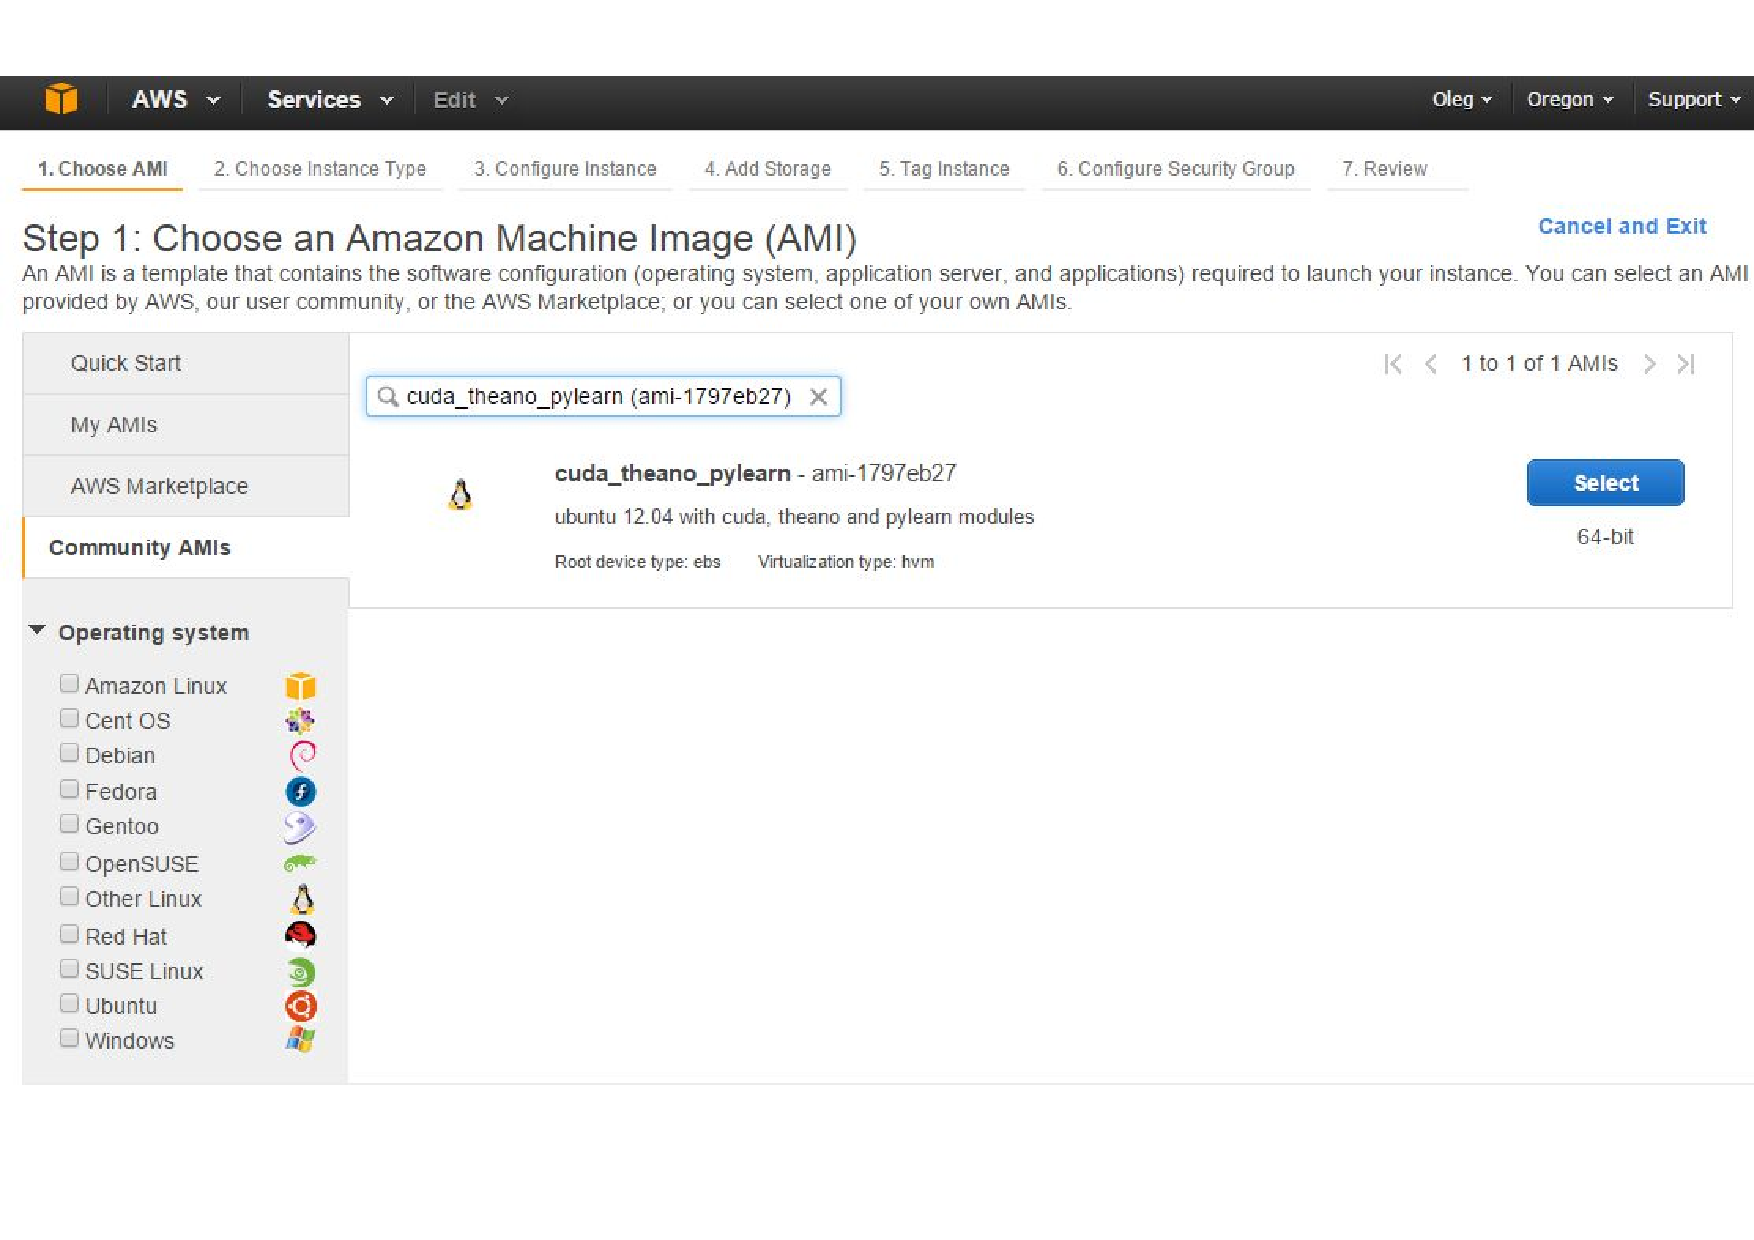
\includegraphics[totalheight=12	cm]{ami.pdf}
 \caption{Выбор конфигурации на консоли AWS}
 \label{fig:ami}
\end{figure}

\begin{figure}[tbph!]
 \centering
  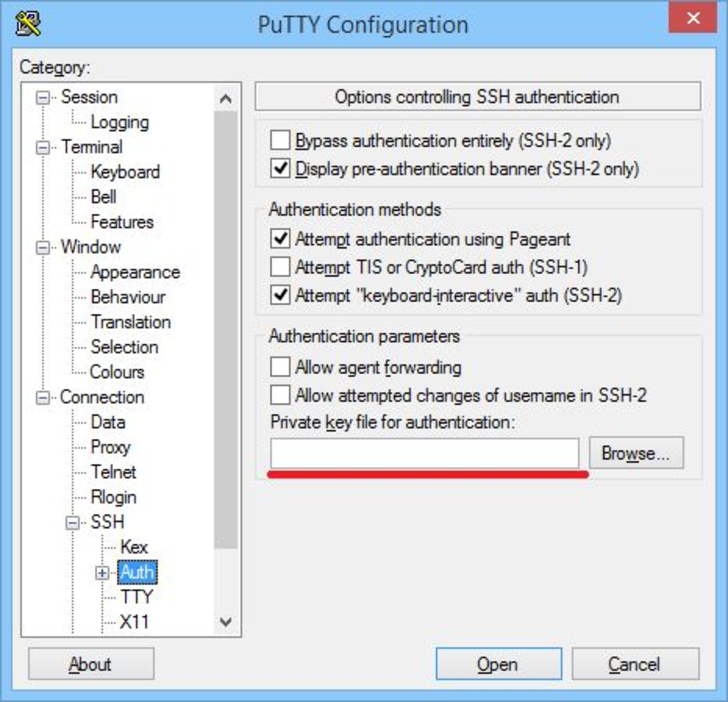
\includegraphics[width=0.5\textwidth]{putty.pdf}
 \caption{Настройка аутентификации Putty}
 \label{fig:putty}
\end{figure}
\begin{figure}[tbph!]
 \centering
  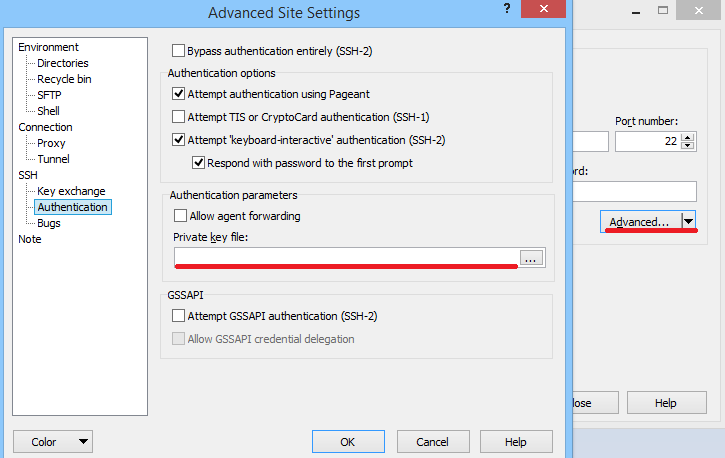
\includegraphics[width=\textwidth]{scp.png}
 \caption{Настройка аутентификации WinSCP}
 \label{fig:scp}
\end{figure}

\subsection{Структура сети глубокого обучения}
Предлагается использовать в качестве алгоритма решения задачи суперпозицию, состоящую из трех основных компонент:
ограниченной машины Больцмана, автокодировщика и двухслойной нейросети с softmax-классификатором.
\paragraph{Ограниченная машина Больцмана.}
Ограниченная машина Больцмана представляет собой двудольный граф, где первая доля соответствует переменной $\mathbf{x}$, а вторая доля --- бинарному вектору $\mathbf{h}$ длины $n'$. 
% \begin{equation}\end{equation}
Рассмотрим случай, когда вектор $\mathbf{x}$ принимает бинарные значения. Определим энергию пары входного слоя $\mathbf{x}$ и скрытого слоя $\mathbf{h}$ следующим образом:
\[
 E(\mathbf{x},\mathbf{h}) = -\mathbf{x}^\text{T} \cdot \mathbf{b}_\text{vis} -\mathbf{h}^\text{T} \cdot \mathbf{b}_\text{hid} - \mathbf{h}^\text{T}\mathbf{W}_\text{RBM}\mathbf{x},
\]
где $\mathbf{b}_\text{vis}, \mathbf{b}_\text{hid}, \mathbf{W}_\text{RBM}$ --- параметры модели.

Пусть совместное распределение пары векторов $\mathbf{x}, \mathbf{h}$ задано следующим образом:
\[
	p(\mathbf{x}, \mathbf{h}) = \frac{1}{Z} \text{exp}\bigl(-E(\mathbf{x},\mathbf{h})\bigr),
\]
где $Z$ --- нормировочный коэффициент:
\[
 Z = \sum_{\mathbf{x} \in \{0,1\}^n, \mathbf{h}\in \{0,1\}^{n'}} \text{exp}\bigl(-E(\mathbf{x},\mathbf{h})\bigr).
\]


Функция вероятностей вектора $\mathbf{x}$ есть сумма вероятностей по всем скрытым состояниям вектора $\mathbf{h}$:
\[
	p(\mathbf{x}) = \sum_{\mathbf{h}\in \{0,1\}^{n'}} p(\mathbf{x}, \mathbf{h}).
\]

Определим элемент суперпозиции~\eqref{eq:main}: \begin{equation}
\label{eq:rbm_model}
\boldsymbol{\mu}_\text{RBM}(\mathbf{x}) = \mathsf{E}(\mathbf{h}|\mathbf{x}).
\end{equation}
Настройка параметров модели ~\eqref{eq:rbm_model} осуществляется решением задачи оптимизации
\begin{equation}
\label{eq:rbm}
\hat{\mathbf{W}}_\text{RBM},\hat{\mathbf{b}}_\text{vis}, \hat{\mathbf{b}}_\text{hid} = \argmax_{{\mathbf{W}_\text{RBM}},{\mathbf{b}}_\text{vis}, {\mathbf{b}}_\text{hid} } p(\mathfrak{D}; {\mathbf{W}},{\mathbf{b}_\text{vis}},{\mathbf{b}_\text{hid}}) = \prod_{\mathbf{x} \in \mathfrak{D}} \sum_{\mathbf{h}\in \{0,1\}^{n'}} \frac{1}{Z} \text{exp}\bigl(-E(\mathbf{\mathbf{x}},\mathbf{h)}\bigr).
\end{equation}
В данной работе используется модифицированная версия ограниченной машины Больцмана, позволяющая работать с небинарными входными данными~\cite{gbrbm}. В этой модификации энергия $E$ пары входного слоя $\mathbf{x}$ и скрытого слоя $\mathbf{h}$ выглядит следующим образом: 
\[
E(\mathbf{x},\mathbf{h}) = \frac{(\mathbf{x} - \mathbf{b}_\text{vis})^2}{2\boldsymbol{\sigma}^2} -\mathbf{h}^\text{T} \cdot \mathbf{b}_\text{hid} - \frac{\mathbf{h}}{\boldsymbol{\sigma}}^\text{T}\mathbf{W}\mathbf{x},
\]
где $\boldsymbol{\sigma}$ --- стандартное нормальное отклонение объектов выборки $\mathfrak{D}$, деление производится покомпонентно.

Для решения задачи оптимизации~\eqref{eq:rbm} используется алгоритм, описанный в~\cite{foundamentals}. 

\paragraph{Автокодировщик.}
Автокодировщик предназначен для снижения размерности исходного пространства признаков. 
Автокодировщик представляет собой суперпозицию кодирующего и декодирующего блока~\cite{foundamentals}:
\[
 \mathbf{\boldsymbol{\mu}}'_\text{AE} = \boldsymbol{\phi}(\mathbf{g}(\mathbf{x})),
\]
где $$\mathbf{g}(\mathbf{x}) = \boldsymbol{\sigma}(\mathbf{W}_\textbf{e}\mathbf{x}+\mathbf{b}_\textbf{e}) \text{ --- кодирующий блок,}$$ 
$$ \boldsymbol{\phi}(\mathbf{g}(\mathbf{x})) = \boldsymbol{\sigma}(\mathbf{W}_\textbf{d}\mathbf{g}(\mathbf{x})+\mathbf{b}_\textbf{d})\text{ --- декодирующий блок,}$$ $$\boldsymbol{\sigma}(\mathbf{t}) = (1+\textbf{exp}({-\mathbf{t}}))^{-1} \text{ --- сигмоидная функция},$$ $\mathbf{W}_\textbf{e},\mathbf{W}_\textbf{d},\mathbf{b}_\textbf{e}, \mathbf{b}_\textbf{d}$ --- параметры модели.

Введем дополнительное ограничение на матрицы $\mathbf{W}_\textbf{e}, \mathbf{W}_\textbf{d}$:
\[
 \mathbf{W}_\textbf{e} = \mathbf{W}_\textbf{d}^{^\text{T}}.
\]

Оптимизацию параметров модели $\mathbf{W}_e$ будем проводить таким образом, чтобы по образу вектора $\mathbf{x}$, получаемому с помощью кодирующего блока, можно было получить вектор $\mathbf{\boldsymbol{\mu}}_\text{AE}$, близкий к исходному входному $\mathbf{x}$, при помощи преобразования декодирующего блока:
\begin{equation}
\label{eq:ae}
 {\hat{\mathbf{W}}}_\textbf{e},\hat{\mathbf{W}}_\textbf{d},\hat{\mathbf{b}}_\textbf{e}, \hat{\mathbf{b}}_\textbf{e} = \argmin_{{\mathbf{W}}_\textbf{e},{\mathbf{W}}_\textbf{d},{\mathbf{b}}_\textbf{e}, {\mathbf{b}}_\textbf{d}} \frac{1}{|\mathfrak{D}|}\sum_{\mathbf{x} \in \mathfrak{D}} ||\mathbf{\boldsymbol{\mu}}_\text{AE}(\mathbf{x})-\mathbf{x}||^2_2.
\end{equation}

Стоит отметить, что декодирующий блок $\boldsymbol{\phi}$ требуется только для решения задачи оптимизации~\eqref{eq:ae} и не используется в суперпозиции ~\eqref{eq:main}. Таким образом, элемент суперпозиции~\eqref{eq:main} определен как
\[
	\mathbf{\boldsymbol{\mu}}_\text{AE} = \mathbf{g}(\mathbf{x}).
\]
\paragraph{Двухслойная нейросеть.}
Двухслойная сеть представляет собой логистическую вектор-функцию~\cite{sm}:
\begin{equation}
\label{sm}
 \mathbf{a}(\mathbf{x}) = \mathbf{W}^\mathsf{T}_2 \textbf{tanh}(\mathbf{W}^\mathsf{T}_1 \mathbf{x}),
\end{equation}
\[
 \mathbf{\boldsymbol{\mu}}_\text{SM}(\mathbf{x}) = \frac{\textbf{exp}\bigl(\mathbf{a}(\mathbf{x})\bigr)}{\sum_{j=1}^Z \text{exp}\bigl({a}_j(\mathbf{x})\bigr)},
\]
где $r$-я компонента вектора $\mathbf{\boldsymbol{\mu}}_\text{SM}(\mathbf{x})$ интерпретируется как вероятность принадлежности объекта $\mathbf{x}$ классу $r$. Итоговая функция классификации~\eqref{eq:main} ставит в соответствие  объекту $\mathbf{x}$ метку класса $y$, где $y$ --- класс, к которому принадлежит $\mathbf{x}$ с наибольшей вероятностью:
$$
 f(\mathbf{w},\mathbf{x})(r) = \begin{cases}
  1,\text{ если }r = \argmax_{r'} {\mu}_\text{SM}(\mathbf{\boldsymbol{\mu}}_\text{AE}(\mathbf{\boldsymbol{\mu}}_\text{RBM}(\mathbf{x}))(r'),\\
  0 \text{ иначе.}
	\end{cases}
$$
где $\mathbf{\boldsymbol{\mu}}_\text{AE}, \mathbf{\boldsymbol{\mu}}_\text{RBM}$ --- автокодировщик~\eqref{eq:ae} и ограниченная машина Больцмана~\eqref{eq:rbm} соответственно, ${\mu}_\text{SM}(\mathbf{x})(r)$ --- $r$-я компонента вектора $ \mathbf{\boldsymbol{\mu}}_\text{SM}$, $f(\mathbf{w},\mathbf{x})(r)$ --- $r$-я компонента вектор-функции $\mathbf{f}$.

Итоговая задача оптимизации выглядит следующим образом:
\[
 \hat{\mathbf{\mathbf{\Theta}}} = \argmin\sum_{\mathbf{x},y \in \mathfrak{D}}\sum_{r = 1}^Z[y = r]\log({\mu}^r_\text{SM}(\mathbf{\boldsymbol{\mu}}_\text{AE}(\mathbf{\boldsymbol{\mu}}_\text{RBM}(\mathbf{x}))),
\]
где $\hat{\mathbf{\mathbf{\Theta}}} = [\hat{\mathbf{W}}_\text{RBM},\hat{\mathbf{b}}_\text{vis},\hat{\mathbf{b}_\text{hid}}, \hat{\mathbf{W}}_\textbf{e}, \hat{\mathbf{b}}_\textbf{e}, \hat{\mathbf{W}^\mathsf{T}_2}, \hat{\mathbf{W}^\mathsf{T}_1}]$ --- параметры ограниченной машины Больцмана~\eqref{eq:rbm}, автокодировщика~\eqref{eq:ae} и двухслойной сети~\eqref{sm}.


\section{Запуск эксперимента на AWS}
В данном разделе кратко изложен порядок действий по запуску вычислительного эксперимента для решения задачи~\eqref{eq:main} на платформе AWS.
\paragraph{Необходимое программное обеспечение.}
Для запуска алгоритма на AWS требуется предварительно зарегистрироваться и активировать аккаунт на сайте AWS. Также следует установить утилиты PUTTY, PUTTYGen и WinSCP для Windows, либо scp и ssh для Linux и Mac OS.
\paragraph{Настройка экземпляра (instance).} Под экземпляром~(англ. instance) AWS понимается предоставляемая сервисом вычислительная платформа, с которой возможно работать как с удаленным сервером. 
После авторизации на странице профиля AWS следует зайти на консоль управления~\cite{console} и выбрать пункт <<EC2>>, ведущий на подраздел <<EC2 Dashboard>>. Для настройки нового экземпляра машины AWS следует нажать кнопку <<Launch Instance>> из этого подраздела. В новом окне будет доступен выбор операционной системы. Для запуска вычислительного эксперимента на Theano наиболее простым вариантом является выбор операционной системы, сконфигурированной сообществом для работы с CUDA и Theano, перечень которых можно найти на вкладке <<Community AMIs>>. Необходимо зайти во вкладку <<Community AMIs>>, в строке поиска ввести имя конфигурации и нажать кнопку <<Select>>.
В данной работе использовалась конфигурация \texttt{<<ami-1797eb27>>}, являющаяся версией операционной системы Ubuntu с предустановленным пакетом Theano (рис.~\ref{fig:ami}).




После выбора конфигурации операционной системы требуется выбрать тип экземпляра и его характеристики: объем жесткого диска, объем оперативной памяти, скорость сети, наличие графического ускорителя и т.~п. В данной работе используется платный тип экземпляра \texttt{g2.2xlarge}, обладающий восьмиядерным процессором, 15 Гб памяти и поддержкой графического ускорителя NVIDIA GRID. В случае если поддержка графического процессора не требуется, можно использовать бесплатный тип экземпляра \texttt{t2.micro}. Дальнейшие настройки экземпляра опциональны. После завершения настройки система предложит создать пару из открытого и закрытого ключа для авторизации в операционной системе экземпляра или выбрать существующий. После завершения настройки экземпляра новый экземпляр появится в таблице на вкладке <<Instances>>, доступной в разделе <<EC2 Dashboard>>. Там же будет доступен и IP-адрес экземпляра (поле <<Public IP>>).


\paragraph{Доступ к экземпляру.}
При работе с экземпляром из операционных систем Linux и Mac OS требуется изменить права для файла ключа:
\begin{quote}
\tt{chmod 400 <путь к ключу>}
\end{quote}

Доступ к экземпляру можно получить по протоколу SSH по адресу, указанному системой после создания экземпляра. 
Для доступа из операционной системы Linux и Mac OS требуется ввести на консоли строку
\begin{quote}
\tt{ssh -i <путь к ключу> ubuntu@<ip-адрес>}
\end{quote}

Для доступа из операционной системы Windows можно использовать программу PuTTY и PuTTYgen. PuTTYgen конвертирует закрытый ключ в приемлемый для AWS вид.
Для конвертации ключа требуется выбрать в программе пункт 
File-Load private key и выбрать полученный от AWS ключ с расширением pem. Затем требуется выбрать кнопку <<Save private key>> и сохранить полученный файл с расширением ppk.

Для дальнейшего использования ключа в Putty требуется выбрать вкладку Connection-SSH-Auth, нажать кнопку <<Browse>> и выбрать ppk-ключ (рис.\ref{fig:putty}). После этого можно заходить на сервер, указав в поле <<Host name>> строку вида
\begin{quote}
\tt{ubuntu@<ip-адрес>}
\end{quote}



\paragraph{Обмен файлами с экземпляром.}
Для обмена файлами с экземпляром можно использовать утилиту scp для Linux и Mac OS и WinSCP для Windows. Как и в случае с соединением по SSH, при работе с экземпляром из операционных систем Linux и Mac OS требуется изменить права для файла ключа:
\begin{quote}
\tt{chmod 400 <путь к ключу>}
\end{quote}

Для копирования данных на сервер экземпляра с использованием утилиты scp требуется ввести на консоли строку
\begin{quote}
\tt{scp -i <ключ> <локальный путь к файлу> ubuntu@<ip-адрес>:<путь к файлу на экземпляре> }
\end{quote}

Для копирования данных с сервера экземпляра на локальный компьютер с использованием утилиты scp требуется ввести на консоли строку
\begin{quote}
\tt{scp -i <путь к ключу> ubuntu@<ip-адрес>:<путь к файлу на экземпляре> <локальный путь к файлу> }
\end{quote}
В случае копирования папки требуется добавить в команде параметр <<-r>>:
\begin{quote}
\tt{scp -i <ключ> -r <локальный путь к папке> ubuntu@<ip-адрес>:<путь к папке на экземпляре> }
\end{quote}

В операционной системе Windows для копирования данных на сервер экземпляра необходимо открыть программу WinSCP. В поле <<Host name>> нужно ввести ip-адрес <<Public IP>>, а в поле <<User name>> -- строку <<ubuntu>>. Затем требуется нажать кнопку <<Advanced>>, в новом окне выбрать вкладку
<<SSH>> --- <<Authentification>>, нажать кнопку <<...>> и выбрать ppk-файл, сгенерированный PuTTYGen (рис.~\ref{fig:scp}). Затем требуется нажать кнопку <<Login>>. После этого можно передавать документы между локальным компьютером и экземпляром AWS.

\paragraph{Завершение работы с экземпляром.}
По завершении работы с экземпляром требуется уничтожить его, выбрав его на консоли управления, и использовав команду <<Terminate>>. \textbf{Важно:} на консоли также имеется команда <<Stop>>, отключающая экземпляр. За хранение данных на отключенном экземпляре может взиматься дополнительная плата. Кроме того, в 2014 году была зафиксирована ошибка AWS, взимавшая дополнительную плату за отключенные инстансы~\cite{bug}, поэтому рекомендуется удалять экземпляр полностью. Также рекомендуется удалить все хранилища данных, присоединенные к экземпляру (вкладка Volumes). 

\paragraph{Запуск вычислительного эксперимента.}
Для запуска вычислительного эксперимента с использованием Theano требуется указать параметры конфигурации Theano перед запуском. В противном случае будет принята конфигурация по умолчанию. Наиболее простым вариантом установки параметров Theano является вызов программы с использованием следующего синтаксиса:
\begin{quote}
\texttt{THEANO\_FLAGS=<параметры Theano в формате <<ключ=значение>> через запятую> python <путь к скрипту>}
\end{quote}

Для запуска скрипта с $n$ процессорами требуется вызвать его следующим образом:
\begin{quote}
\texttt{OMP\_NUM\_THREADS=n python <путь к скрипту>}
\end{quote}

Для запуска скрипта с использованием CUDA требуется вызвать скрипт следующей командой:
\begin{quote}
\texttt{THEANO\_FLAGS=device=gpu,floatX=float32 python <путь к скрипту> }
\end{quote}
Здесь \texttt{ floatX=float32 } --- параметр, отвечающий за формат вещественных чисел при обработке Theano. В настоящее время при работе с CUDA поддерживается только float32. 

\paragraph{Общий план запуска алгоритма.}
Ниже приведена общая пошаговая инструкция запуска алгоритма на сервере AWS.

\begin{itemize}
\item Зарегистрироваться на AWS,
\item сконфигурировать экземпляр,
\item скопировать код и данные проекта на сервер (например, в папку \texttt{/home/ubuntu/}),
\item присоединиться к серверу по протоколу SSH,
\item зайти в папку с проектом с использованием команды cd,
\item запустить вычислительный эксперимент,
\item скопировать результаты эксперимента на локальный компьютер,
\item уничтожить экземпляр.
\end{itemize}

В качестве примера запуска вычислительного эксперимента можно вызвать команду
\texttt{sh run8CPU.sh}
для запуска эксперимента на восьми ядрах процессора или 
\texttt{sh runGPU.sh}
для запуска эксперимента на графическом ускорителе. Подробно параметры запуска описаны в Readme-файле проекта~\cite{svn}.
\section{Построение сети глубокого обучения заданной структуры на языке Matlab}
В качестве независимого варианта решения задачи~\eqref{eq:main} предлагается использовать инструментарий~\cite{source_popova} авторов~\cite{ts3} на языке Matlab. Он предназначен для построения нейронных сетей глубокого обучения со структурой, задаваемой пользователем. 
\paragraph{Описание процедуры запуска инструментария.} Для настройки и тестирования сети необходим набор данных. Данные должны быть сохранены в формате csv (comma separated values), а файл должен быть назван dataset.csv. Файл dataset.csv состоит из $N$ числовых строк. Первое число в каждой строке файла должно быть целым числом от 1 до $Z$ -- это метка класса. Оставшиеся $m$ чисел в строке -- это числовые признаки объекта~\eqref{eq:dataset}. Далее необходимо задать желаемую структуру модели. Для этого нужно создать файл model.csv. Этот файл состоит из одной числовой строки. Первое число~$K$ --- это желаемое число уровней суперпозиции модели. Следующие $K$ чисел -- описание типов уровней (1 -- ограниченная машина Больцмана, 2 -- автокодировщик, 3 -- двухслойная нейросеть), следующие $K$ чисел -- число нейронов в каждом слое с первого по K-й соответственно, следующие $K$ чисел -- число циклов обучения для каждого слоя. Последнее число в строке -- число объектов выборки, которые будут случайным образом выбраны из всего набора данных для обучения модели. \\

Пример. Строка $3~1~2~3~100~80~50~100~100~200~500$ описывает следующую модель: трехслойная суперпозиция ограниченной машины Больцмана со 100 нейронами, автокодировщика с 80 нейронами и двухслойной нейросети с 50 нейронами. Для обучения модели случайным образом будет выбрана подвыборка мощности 500. Будет проведено 100 циклов обучения RBM, 100 циклов обучения автокодировщика и 200 циклов обучения двухслойной нейросети.\\

Замечание. Ограниченные машины Больцмана и автокодировщики обучаются <<без учителя>> и задают процедуру порождения признаков, т.~е. на выходе этих моделей получается преобразованная матрица признакового описания. Двухслойная нейросеть обучается <<с учителем>> и непосредственно разделяет объекты на классы. Учитывая это, структура $K$-слойной модели должна быть задана таким образом, чтобы первые $K-1$ слоев состояли из машин Больцмана и автокодировщиков, а последний слой -- из двухслойной нейросети.

\paragraph{Настройка нейронной сети.} После подготовки файлов с набором данных и описанием суперпозиции можно создать, обучить и протестировать модель. Для этого необходимо выполнить следующие шаги:
\begin{enumerate}[1)]
\item загрузить на компьютер инструментарий из репозитория MLAlgorithms~\cite{source_popova};
\item запустить систему Matlab;
\item в качестве рабочей директории в Matlab установить директорию \\$\dots\backslash \text{Popova2015Deeplearning}$;
\item поместить файл dataset.csv в папке $\dots\backslash \text{Popova2015Deeplearning}\backslash \text{data}$, а файл model.csv в папку $\dots\backslash \text{Popova2015Deeplearning}\backslash \text{code}$;
\item запустить файл main.m, который находится в папке $\dots\backslash \text{Popova2015Deeplearning}\backslash \text{code}$.

\end{enumerate}

После того как файл main.m завершит работу в папке $\dots\backslash \text{Popova2015Deeplearning}\backslash \text{report}$ будут сохранены графики c ROC-кривой и функционалом AUC, а также файл model.mat, в котором хранится настроенная модель.


\section{Вычислительный эксперимент}
В качестве данных для проведения вычислительного эксперимента использовались данные WISDM~\cite{wisdm}, представляющие собой набор записей акселерометра мобильного телефона. Каждой записи соответствуют три координаты по осям акселерометра. Набор данных содержит записи движений для 6 классов переменной длины.
При проведении вычислительного эксперимента из каждой записи использовались первые 200 сегментов. Т.~к. выборка не сбалансирована, в нее добавлялись повторы записей классов, содержащих количество записей, меньшее чем у большего класса.

Основные эксперименты --- исследование зависимости ошибки классификации от числа параметров и размера выборки --- были проведены как с использованием инструментария на базе библиотеки Theano, так и с использованием инструментария на языке Matlab. 
Для оценки качества классификации была проведена процедура скользящего контроля~\cite{cv} при соотношении количества объектов обучающей и контрольной выборки 3:1. Число нейронов на каждом слое задавалось из соотношения 10:6:3. При проведении процедуры скользящего контроля для каждого отсчета количества нейронов было произведено пять запусков. В эксперименте с использованием инструментария на базе Theano при обучении двухслойной нейронной сети проводился мультистарт~\cite{multi}, т.~е. одновременный запуск обучения сети с 8 разными стартовыми значениями параметров для предотвращения возможного застревания алгоритма обучения в локальном минимуме. При оценке качества классификации выбиралась модель с наилучшими результатами. График зависимости ошибки классификации от числа используемых нейронов изображен на рис.~\ref{fig:neurons}.

\begin{figure}[tb!]
 \centering
  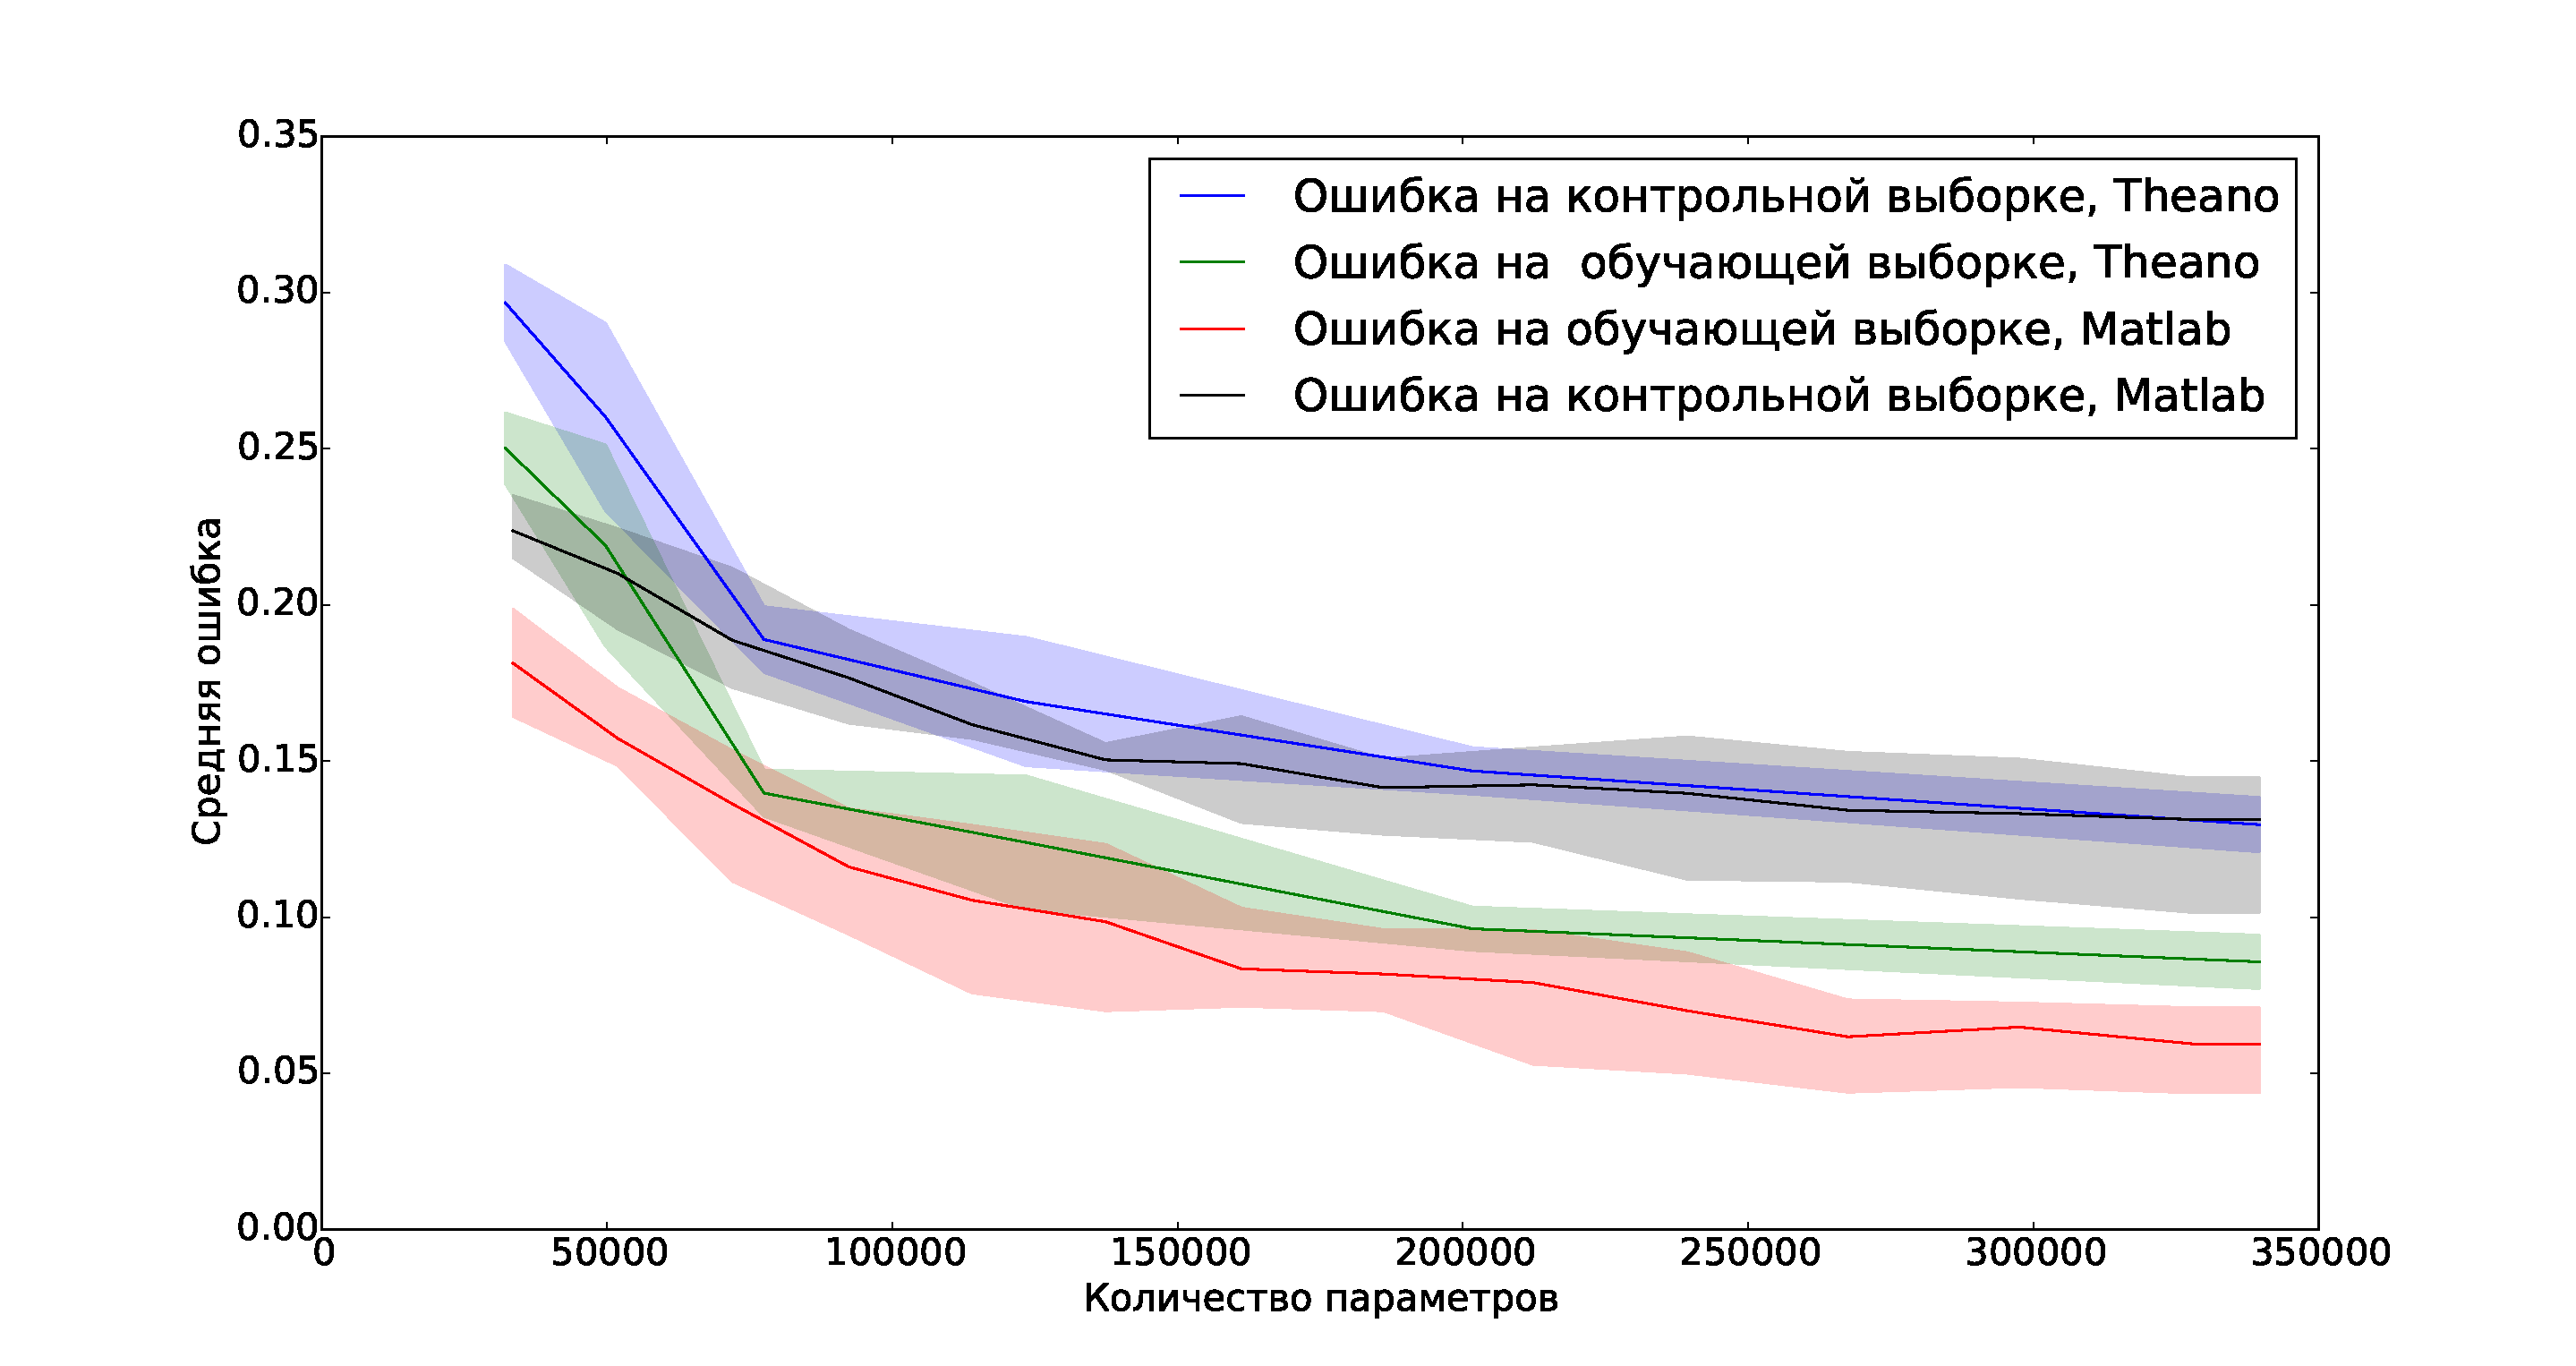
\includegraphics[width=1.0\textwidth]{neurons.pdf}
 \caption{Зависимость ошибки от числа нейронов}
 \label{fig:neurons}
\end{figure}


Для оценки зависимости качества классификации от размера обучающей выборки была проведена кроссвалидация с фиксированным количеством объектов в обучающей выборке (25\% исходной выборки) и переменным размером обучающей выборки. Число нейронов было установлено как 364:224:112. При проведении процедуры скользящего контроля для каждого отсчета было произведено пять запусков. График зависимости ошибки классификации от размера обучающей выборки представлен на рис.~\ref{fig:samples}.


\begin{figure}[tb!]
 \centering
  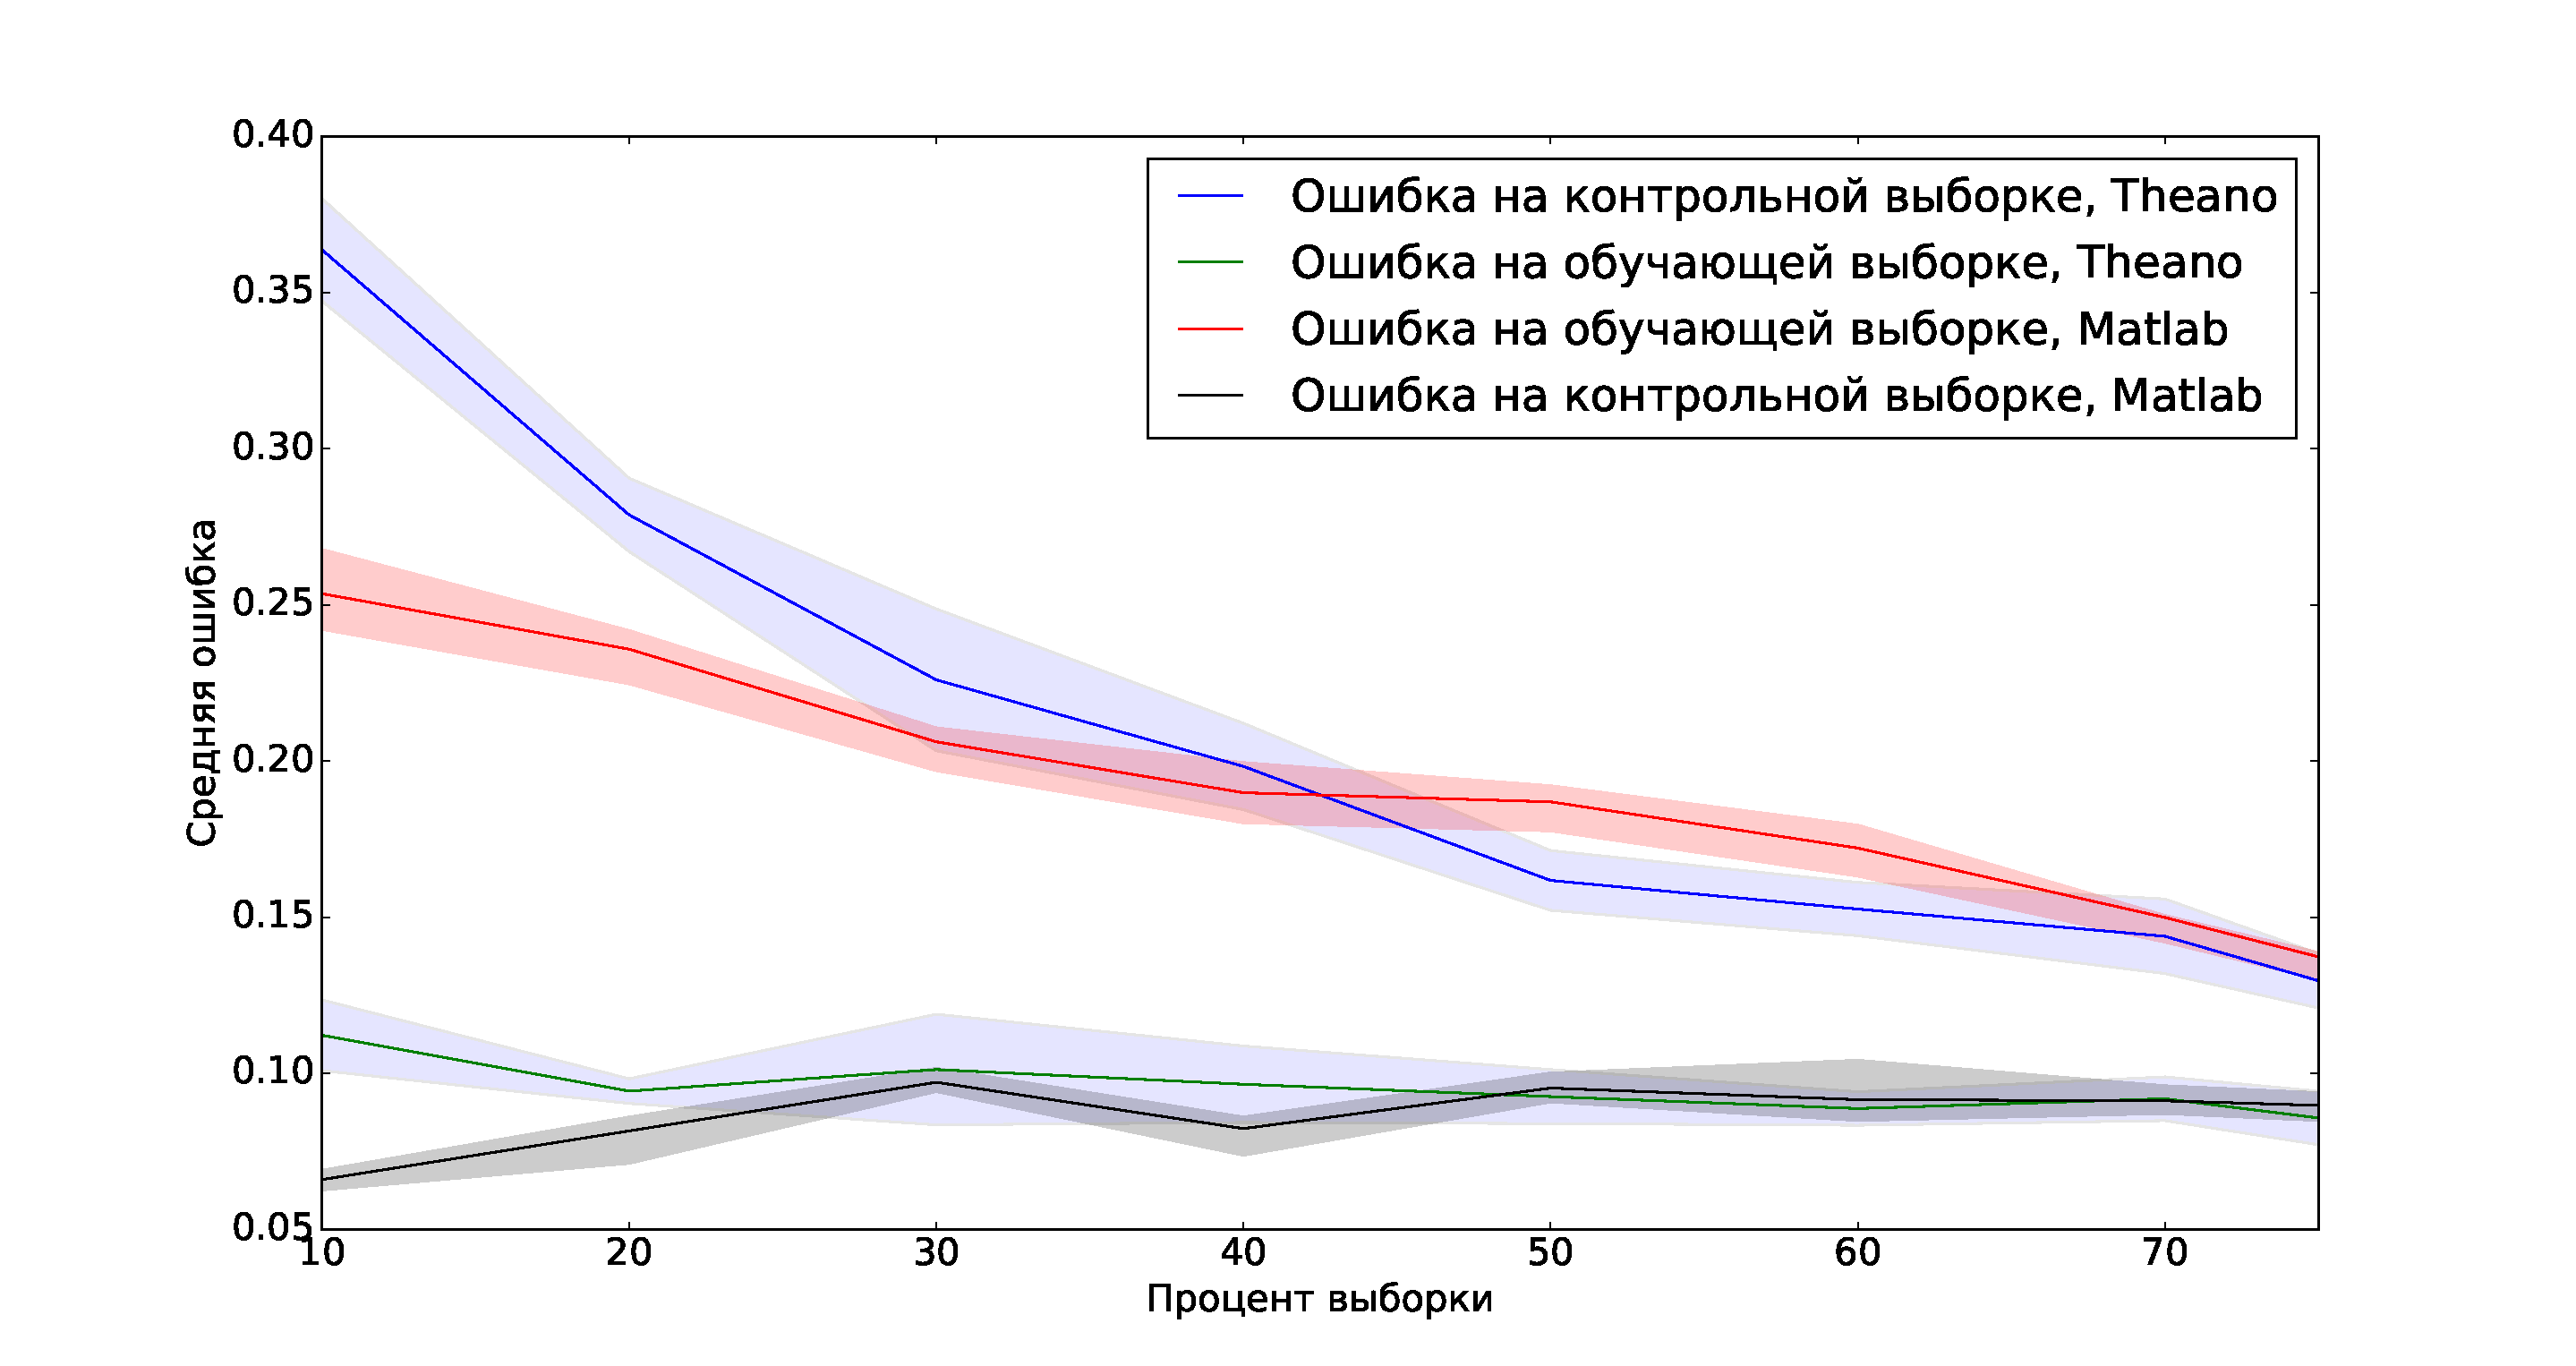
\includegraphics[width=1.0\textwidth]{samples.pdf}
 \caption{Зависимость ошибки от размера обучающей выборки}
 \label{fig:samples}
\end{figure}


Для исследования скорости процесса обучения нейросети в зависимости от конфигурации Theano был сделан следующий эксперимент:
проводилось обучение двухслойной нейросети на основе подсчитанных заранее параметров ограниченной машины Больцмана~\eqref{eq:rbm} и автокодировщика~\eqref{eq:ae}. Обучение проходило за 100 итераций. При обучении алгоритм запускался параллельно с $n$ разными стартовыми позициями, $n \in \{1,\dots,4\}.$ Число нейронов было установлено как 300:200:100.
Запуск осуществлялся со следующими конфигурациями Theano:
\begin{itemize}
\item вычисление на центральном процессоре, задействовано 
одно ядро;
\item вычисление на центральном процессоре, задействовано четыре ядра;
\item вычисление на центральном процессоре, задействовано восемь ядер;
\item вычисление на графическом процессоре.
\end{itemize}

Результаты эксперимента приведены на рис.~\ref{fig:speed}. Как видно из графика, вычисление с использованием CUDA показывает значительное ускорение по сравнению с вычислением на центральном процессоре.

\begin{figure}[tb!]
 \centering
  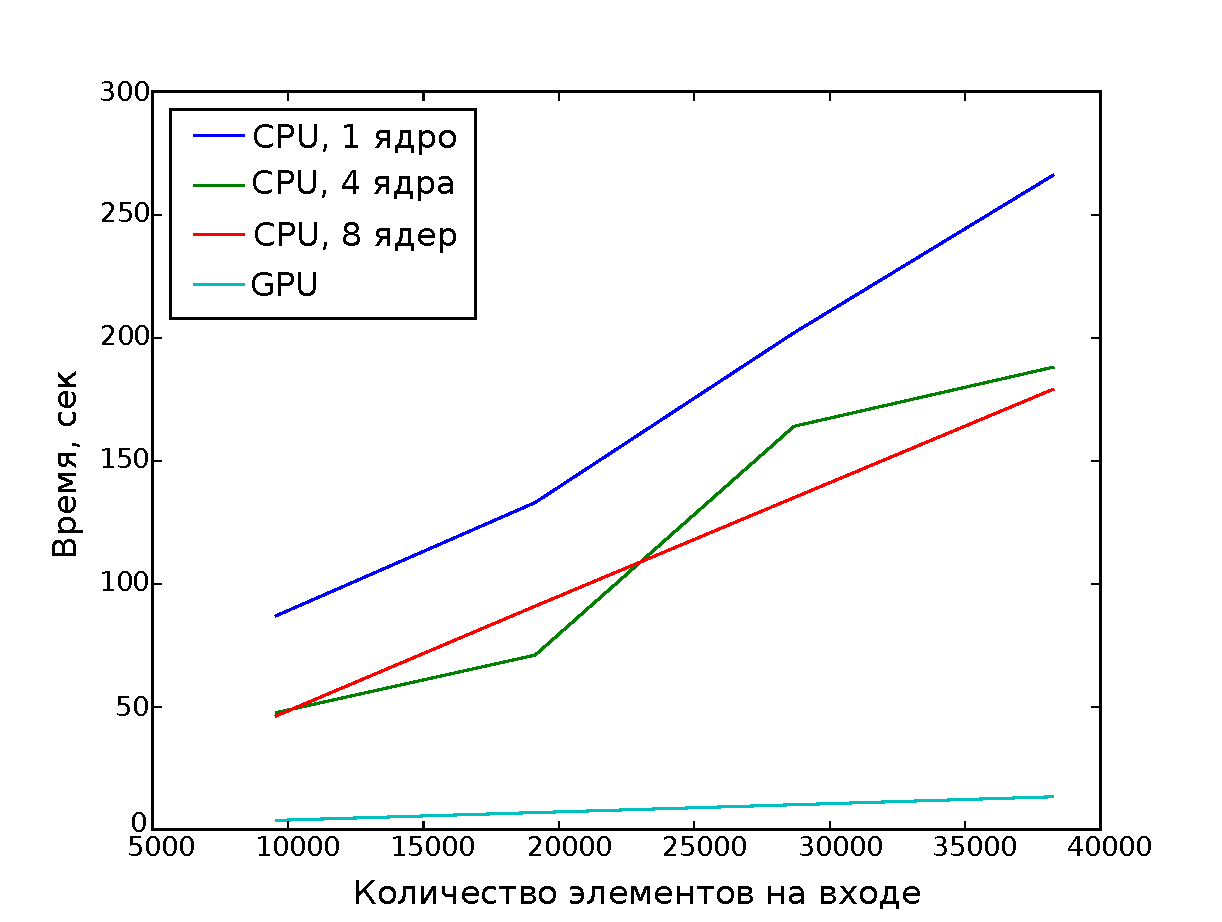
\includegraphics[width=0.8\textwidth]{result.pdf}
 \caption{Результаты эксперимента по исследованию скорости процесса обучения}
 \label{fig:speed}
\end{figure}

\section{Заключение}
В данной работе был проведен ряд вычислительных экспериментов с использованием библиотеки Theano и сервисом облачных вычислений Amazon WebService. Проведены эксперименты для установления зависимости ошибки классификации временных рядов с использованием сетей глубокого обучения от размера выборки и числа параметров сети. Исследовалась эффективность обучения искусственной нейросети с использованием графического процессора. Эксперимент показал значительное ускорение вычислений на графическом процессоре. Исходный код экспериментов доступен по адресам~\cite{svn,source_popova}.




\begin{thebibliography}{10}
\def\selectlanguageifdefined#1{
\expandafter\ifx\csname date#1\endcsname\relax
\else\language\csname l@#1\endcsname\fi}
\ifx\undefined\url\def\url#1{{\small #1}}\else\fi
\ifx\undefined\BibAuthor\def\BibAuthor#1{\emph{#1}}\else\fi
\ifx\undefined\BibTitle\def\BibTitle#1{#1}\else\fi
\ifx\undefined\BibUrl\def\BibUrl#1{\url{#1}}\else\fi
\ifx\undefined\BibAnnote\def\BibAnnote#1{}\else\fi
\ifx\undefined\BibSection\def\BibSection#1#2#3{}\else\fi

\bibitem{foundamentals}
 {Cho K.}
{Foundations and Advances in Deep Learning}. Espoo: Aalto University, 2014. Doctoral dissertation.

%http://www.diva-portal.org/smash/get/diva2:710518/FULLTEXT02
\bibitem{ts1}
 {Längkvist M.,  Karlsson L., Loutfi A.}
A review of unsupervised feature learning for time-series modelling //{Pattern Recognition Letters}, 2014. Vol. 42(1). P. 11-24. 

%http://tdesell.cs.und.edu/papers/2015_evocop.pdf
\bibitem{ts2}
 {Desell T., Clachar S.,  Higgins J., Wild B.}
Evolving Deep Recurrent Neural Networks Using Ant
Colony Optimization // {Evolutionary Computation in Combinatorial Optimization}, 2015. Vol. 9026. P. 86-98. 


\bibitem{ts3}
 {Popova M. S.,  Strijov V. V.}
Building superposition of deep learning neural networks
for solving the problem of time series classification // {Systems and Means of Informatics}, 2015. Vol. 25(3). P. 60-77.


http://www.cs.toronto.edu/~hinton/absps/JMLRdropout.pdf
\bibitem{reg1}
{Srivastava N.,  Hinton G.,  Krizhevsky A.,  Sutskever I.,  Salakhutdinov R. }
Dropout: A Simple Way to Prevent Neural Networks from
Overfitting // {Journal of Machine Learning Research}, 2014. Vol. 15. P. 1929-1958.

http://papers.nips.cc/paper/4882-dropout-training-as-adaptive-regularization.pdf
\bibitem{reg2}
{Wager S., Wang S.,  Liang P.}
Dropout Training as Adaptive Regularization // {Advances in Neural Information Processing Systems}, 2013. Vol. 26. P.{351-359}. 

%http://arxiv.org/pdf/1506.02142v1.pdf
\bibitem{reg3}
{Gal Y.,  Ghahramani Z.}
Dropout as a Bayesian Approximation:
Representing Model Uncertainty in Deep Learning. 2015. URL: http://arxiv.org/abs/1506.02142.

%Regularization of Neural Networks using DropConnect
\bibitem{reg4}
{Wan L., Zeiler M.,  Zhang S., LeCun Y.,  Fergus R. }
Regularization of Neural Networks using DropConnect //{Proceedings of the 30th International Conference on Machine Learning (ICML-13)}, 2013. P. 1058-1066.


%http://arxiv.org/pdf/1312.6199v4.pdf
\bibitem{stab1}
{Szegedy C., 
Zaremba W.,
Sutskever I., 
Bruna J., 
Erhan D., 
Goodfellow I.,
Fergus R.}
Intriguing properties of neural networks. 2014. URL: http://arxiv.org/abs/1312.6199.

%http://ai.stanford.edu/~ang/papers/nips09-MeasuringInvariancesDeepNetworks.pdf
\bibitem{stab2}
{Goodfellow I. J., Le Q. V., Saxe A. M., Lee H., Ng A. Y.}
Measuring Invariances in Deep Networks //{Advances in Neural Information Processing Systems}, 2009. Vol. 22. P. 646-654.


%http://machinelearning.wustl.edu/mlpapers/paper_files/AISTATS2012_RaikoVL12.pdf
\bibitem{speed1}
{Raiko T.,  Valpola H., LeCun Y.}
Deep Learning Made Easier by Linear Transformations in
Perceptrons //{Journal of Machine Learning Research - Workshop and Conference Proceedings}, 2012. Vol. 22. P. 924-932.

%http://arxiv.org/pdf/1306.1091.pdf
\bibitem{speed2}
{Bengio Y.,  Laufer E., Alain G.,  Yosinski G. }
Deep Generative Stochastic Networks Trainable by Backprop //{Proceedings of The 31st International Conference on Machine Learning}, 2014. P. 226–234.


%http://arxiv.org/pdf/1502.03167.pdf
\bibitem{speed3}
{Ioffe S., Szegedy C.}
Batch Normalization: Accelerating Deep Network Training by Reducing Internal Covariate Shift. 2015. URL: http://arxiv.org/abs/1502.03167.

%http://www.cv-foundation.org/openaccess/content_cvpr_2013/papers/Li_Learning_Locally-Adaptive_Decision_2013_CVPR_paper.pdf
\bibitem{ada}
{Li Z.,  Chang C., Liang F., Huang T. S.,  Cao C.,  Smith J. R.}
Learning Locally-Adaptive Decision Functions for Person Verification //{Computer Vision and Pattern Recognition (CVPR), 2013 IEEE Conference on}, 2013. P. 3610-3617.

%http://www.uoguelph.ca/~gwtaylor/publications/nips2008/rtrbm.pdf
\bibitem{recrbm}
{Sutskever I.,  Hinton G.,  Taylor G.}
The Recurrent Temporal Restricted Boltzmann
Machine //{Advances in Neural Information Processing Systems}, 2009. Vol. 21. P. 1601--1608.

%ahttp://image.diku.dk/igel/paper/TRBMAI.pdf
\bibitem{rbm}
 {Fischer F., Igel C.}
Training Restricted Boltzmann Machines: An Introduction //{Pattern Recognition}, 2014. Vol. 47. P. 25-39.

%http://papers.nips.cc/paper/4204-dynamic-pooling-and-unfolding-recursive-autoencoders-for-paraphrase-detection.pdf
\bibitem{rae}
{Socher R.,  Huang E. H.,  Pennington J.,  Ng A. Y., Manning C. D. }
Dynamic Pooling and Unfolding Recursive Autoencoders for Paraphrase Detection //{Advances in Neural Information Processing Systems 24}, 2011. P. 801--809.



%Sparse Autoencoders for Word Decoding from Magnetoencephalography
\bibitem{sparse}
{Shu M.,  Fyshe F.}
Sparse Autoencoders for Word Decoding from Magnetoencephalography. 2013. URL: http://www.cs.cmu.edu/$\sim$afyshe/papers/SparseAE.pdf.

%http://www.jmlr.org/papers/volume11/vincent10a/vincent10a.pdf
\bibitem{denoise}
{Vincent P., Larochelle H., Lajoie I., Bengio Y., Manzagol P.}
Stacked Denoising Autoencoders: Learning Useful Representations in
a Deep Network with a Local Denoising Criterion //{The Journal of Machine Learning Research}, 2013. Vol. 11. P. 3371-3408.




\bibitem{wisdm}
{Kwapisz J. R., Weiss G. M.,  Moore S.}
Activity recognition using cell phone
accelerometers // \emph{SIGKDD Explorations}, 2010. Vol. 12(2). P. 74-82.

%. “Theano: new features and speed improvements”. NIPS 2012 deep learning workshop. (BibTex)
\bibitem{theano1}
{Bastien F., Lamblin P., Pascanu R., Bergstra J., Goodfellow I., Bergeron A., Bouchard N., Warde-Farley D.,  Bengio Y.}
Theano: new features and speed improvements. 2012. URL:  http://arxiv.org/pdf/1211.5590v1.pdf.

%J. Bergstra, O. Breuleux, F. Bastien, P. Lamblin, R. Pascanu, G. Desjardins, J. Turian, D. Warde-Farley and Y. Bengio. “Theano: A CPU and GPU Math Expression Compiler”. Proceedings of the Python for Scientific Computing Conference (SciPy) 2010. June 30 - July 3, Austin, TX (BibTeX)
\bibitem{theano2}
{Bergstra J., Breuleux O., Bastien F., Lamblin P., Pascanu R., Desjardins G., Turian J., Warde-Farley D., Bengio Y.}
Theano: a {CPU} and {GPU} Math Expression Compiler //{Proceedings of the Python for Scientific Computing Conference ({SciPy})}, 2010. P. 3-11.
%
\bibitem{pylearn}
{Goodfellow I. J.,  Warde-Farley D., Lamblin P., Dumoulin V., Mirza M., Pascanu R., Bergstra J., Bastien F., Bengio Y.}
Pylearn2: a machine learning research library. 2013. URL: http://arxiv.org/abs/1308.4214.
%
\bibitem{lasagne}
{Dieleman S., Schlüter J.,  Raffel C. et al.}
{Lasagne: First release.} 2015. URL: http://dx.doi.org/10.5281/zenodo.27878.

\bibitem{cuda}
%https://devtalk.nvidia.com/default/topic/521083/canonical-citation-reference-for-cuda/
{Nickolls J.,  Buck I., Garland M. Skadron K.}
Scalable Parallel Programming with CUDA //{ACM Queue}, 2008. Vol. 6(2). P. 40-53.

%http://dl.acm.org/citation.cfm?id=1803953
\bibitem{cl}
{Stone  J. E.,   Gohara D.,  Shi G.}
OpenCL: A Parallel Programming Standard for Heterogeneous Computing Systems
//{Journal
IEEE Design \& Test}, 2010. Vol. 12(10). P. 66-73.

%http://jmlr.org/papers/volume11/erhan10a/erhan10a.pdf
\bibitem{fine}
{Erhan D., 
Bengio Y.,
Courville A.,
Manzagol P.,
Vincent P.}
Why Does Unsupervised Pre-training Help Deep Learning? //{The Journal of Machine Learning Research}, 2010. Vol. 11. P. 625-660.


%http://www.gatsby.ucl.ac.uk/~chuwei/paper/smc.pdf
\bibitem{nnl}
{ Duan K., Keerthi S. S., Chu W.,  Shevade S. K., Poo A. N.}
Multi-Category Classification by Soft-Max
Combination of Binary Classifiers //{The
fourth international workshop on multiple classifier systems}, 2003. P. 125-134.


%https://users.ics.aalto.fi/praiko/papers/nips11Cho.pdf
\bibitem{gbrbm}
{Cho K.,  Raiko T.,  Ilin A.}
Gaussian-Bernoulli Deep Boltzmann Machine //{The 2013 International Joint Conference on Neural Networks (IJCNN)}, 2013. P. 1-7. 

%http://www.mitpressjournals.org/doi/pdf/10.1162/neco.2006.18.7.1527
\bibitem{sm}
{Hinton G. E.,  Osindero S., Teh Y.}
A Fast Learning Algorithm for Deep Belief Nets //{Neural Computation}, 2006. Vol. 18. P. 1527–1554.

%http://stackoverflow.com/questions/2549035/do-you-get-charged-for-a-stopped-instance-on-ec2
\bibitem{bug}
URL: http://stackoverflow.com/questions/2549035/do-you-get-charged-for-a-stopped-instance-on-ec2.

%
\bibitem{console}
URL: https://us-west-2.console.aws.amazon.com/console/.
%
\bibitem{cv}
{Bishop, C. M.}
Pattern Recognition and Machine Learning. --- eds. 2006 --- Springer-Verlag New York. 738 p.


%URL:http://www.researchgate.net/profile/Marco_Locatelli/publication/227102777_Machine_learning_for_global_optimization/links/0c96053b561d2cf6c1000000.pdf
\bibitem{multi}
{Cassioli A., Lorenzo D. D., Locatelli M., Schoen F., Sciandrone M.}
Machine Learning for Global Optimization //{Computational Optimization and Applications}, 2012. Vol. 1(1). P. 279-303.

%
\bibitem{svn}
URL: \\ https://svn.code.sf.net/p/mlalgorithms/code/Group074/\\Bakhteev2015TheanoCuda/code/.

%
\bibitem{source_popova}
URL: \\https://svn.code.sf.net/p/mlalgorithms/code/Group174/\\Popova2015DeepLearning/.
\end{thebibliography}



\renewcommand\refname{References}
\begin{thebibliography}{10}
\def\selectlanguageifdefined#1{
\expandafter\ifx\csname date#1\endcsname\relax
\else\language\csname l@#1\endcsname\fi}
\ifx\undefined\url\def\url#1{{\small #1}}\else\fi
\ifx\undefined\BibAuthor\def\BibAuthor#1{\emph{#1}}\else\fi
\ifx\undefined\BibTitle\def\BibTitle#1{#1}\else\fi
\ifx\undefined\BibUrl\def\BibUrl#1{\url{#1}}\else\fi
\ifx\undefined\BibAnnote\def\BibAnnote#1{}\else\fi
\ifx\undefined\BibSection\def\BibSection#1#2#3{}\else\fi

\bibitem{foundamentals}
 {Cho, K.}
2014. Doctoral dissertation {Foundations and Advances in Deep Learning}. Espoo: Aalto University. 277 p.

%http://www.diva-portal.org/smash/get/diva2:710518/FULLTEXT02
\bibitem{ts1}
 {Längkvist, M., L. Karlsson and A. Loutfi.}
2014. A review of unsupervised feature learning for time-series modelling. \emph{Pattern Recognition Letters}. 42(1): 11-24. 

%http://tdesell.cs.und.edu/papers/2015_evocop.pdf
\bibitem{ts2}
 {Desell, T., S. Clachar, J. Higgins and B. Wild.}
2015. Evolving Deep Recurrent Neural Networks Using Ant
Colony Optimization. \emph{Evolutionary Computation in Combinatorial Optimization}. 9026: 86-98. 

\bibitem{ts3}
 {Popova, M. S. and V. V. Strijov}
2015. Building superposition of deep learning neural networks
for solving the problem of time series classification. \emph{Systems and Means of Informatics}. 25(3): 60-77.


%http://www.cs.toronto.edu/~hinton/absps/JMLRdropout.pdf
\bibitem{reg1}
{Srivastava, N., G. Hinton, A. Krizhevsky, I. Sutskever and R. Salakhutdinov. }
2014. Dropout: A Simple Way to Prevent Neural Networks from
Overfitting. \emph{Journal of Machine Learning Research}. 15: 1929-1958.

%http://papers.nips.cc/paper/4882-dropout-training-as-adaptive-regularization.pdf
\bibitem{reg2}
{Wager, S., S. Wang and P. Liang.}
2013. Dropout Training as Adaptive Regularization. \emph{Advances in Neural Information Processing Systems}. \mbox{26:~{351-359}}. 

%http://arxiv.org/pdf/1506.02142v1.pdf
\bibitem{reg3}
{Gal, Y. and Z. Ghahramani}
2015. Dropout as a Bayesian Approximation:
Representing Model Uncertainty in Deep Learning. \emph{arXiv preprint arXiv:1506.02142}. Available At: http://arxiv.org/abs/1506.02142 (accessed November 25, 2015).

%Regularization of Neural Networks using DropConnect
\bibitem{reg4}
{Wan, L., M. Zeiler, S. Zhang, Y. LeCun and R. Fergus. }
2013. Regularization of Neural Networks using DropConnect. \emph{Proceedings of the 30th International Conference on Machine Learning (ICML-13)}. 1058-1066.


%http://arxiv.org/pdf/1312.6199v4.pdf
\bibitem{stab1}
{Szegedy, C., 
W. Zaremba,
I. Sutskever, 
J. Bruna, 
D. Erhan, 
I. Goodfellow and 
R. Fergus.}
2014. Intriguing properties of neural networks.  \emph{arXiv preprint arXiv:1312.6199}. Available At: http://arxiv.org/abs/1312.6199 (accessed November 25, 2015).

%http://ai.stanford.edu/~ang/papers/nips09-MeasuringInvariancesDeepNetworks.pdf
\bibitem{stab2}
{Goodfellow, I. J., Q. V. Le, A. M. Saxe, H. Lee and A. Y. Ng.}
2009. Measuring Invariances in Deep Networks. \emph{Advances in Neural Information Processing Systems}. 22: 646--654.


%http://machinelearning.wustl.edu/mlpapers/paper_files/AISTATS2012_RaikoVL12.pdf
\bibitem{speed1}
{Raiko, T., H. Valpola and Y. LeCun.}
2012. Deep Learning Made Easier by Linear Transformations in
Perceptrons. \emph{Journal of Machine Learning Research - Workshop and Conference Proceedings}. 22: 924-932.

%http://arxiv.org/pdf/1306.1091.pdf
\bibitem{speed2}
{Bengio, Y., E. Laufer, G. Alain and G. Yosinski. }
2014. Deep Generative Stochastic Networks Trainable by Backprop. \emph{Proceedings of The 31st International Conference on Machine Learning}. 226–234.


%http://arxiv.org/pdf/1502.03167.pdf
\bibitem{speed3}
{Ioffe, S. and C. Szegedy.}
2015. Batch Normalization: Accelerating Deep Network Training by Reducing Internal Covariate Shift. \emph{arXiv preprint arXiv:1502.03167}. Available At: http://arxiv.org/abs/1502.03167 (accessed November 25, 2015).

%http://www.cv-foundation.org/openaccess/content_cvpr_2013/papers/Li_Learning_Locally-Adaptive_Decision_2013_CVPR_paper.pdf
\bibitem{ada}
{Li, Z., C. Chang, F. Liang, T. S. Huang, C. Cao and J. R. Smith.}
2013. Learning Locally-Adaptive Decision Functions for Person Verification. \emph{Computer Vision and Pattern Recognition (CVPR), 2013 IEEE Conference on}. 3610-3617.

%http://www.uoguelph.ca/~gwtaylor/publications/nips2008/rtrbm.pdf
\bibitem{recrbm}
{Sutskever, I., G. Hinton and G. Taylor.}
2009. The Recurrent Temporal Restricted Boltzmann
Machine. \emph{Advances in Neural Information Processing Systems}. 21: 1601--1608.

%ahttp://image.diku.dk/igel/paper/TRBMAI.pdf
\bibitem{rbm}
 {Fischer, A. and C. Igel.}
2014. Training Restricted Boltzmann Machines: An Introduction. \emph{Pattern Recognition}. 47:~25-39.

%http://papers.nips.cc/paper/4204-dynamic-pooling-and-unfolding-recursive-autoencoders-for-paraphrase-detection.pdf
\bibitem{rae}
{Socher, R., E. H. Huang, J. Pennington, A. Y. Ng and C. D. Manning. }
2011. Dynamic Pooling and Unfolding Recursive Autoencoders for Paraphrase Detection. \emph{Advances in Neural Information Processing Systems 24}. 801--809.



%Sparse Autoencoders for Word Decoding from Magnetoencephalography
\bibitem{sparse}
{Shu, M. and F. Fyshe.}
2013. Sparse Autoencoders for Word Decoding from Magnetoencephalography. \emph{Proceedings of the third NIPS Workshop on Machine Learning and Interpretation in NeuroImaging (MLINI)}. Available at: http://www.cs.cmu.edu/$\sim$afyshe/papers/SparseAE.pdf
(accessed November 25, 2015).

%http://www.jmlr.org/papers/volume11/vincent10a/vincent10a.pdf
\bibitem{denoise}
{Vincent, P., H. Larochelle, I. Lajoie, Y. Bengio and 
P. Manzagol.}
2013. Stacked Denoising Autoencoders: Learning Useful Representations in
a Deep Network with a Local Denoising Criterion. \emph{The Journal of Machine Learning Research}. 11: 3371-3408.




\bibitem{wisdm}
{Kwapisz, J. R., G. M. Weiss and S. Moore.}
2010. Activity recognition using cell phone
accelerometers. \emph{SIGKDD Explorations}. 12(2): 74-82.

%. “Theano: new features and speed improvements”. NIPS 2012 deep learning workshop. (BibTex)
\bibitem{theano1}
{Bastien, F., P. Lamblin, R. Pascanu, J. Bergstra, I. Goodfellow, A. Bergeron, N. Bouchard, D. Warde-Farley and Y. Bengio.}
2012. Theano: new features and speed improvements. \emph{Deep Learning and Unsupervised Feature Learning NIPS 2012 Workshop}. Available at:  http://arxiv.org/pdf/1211.5590v1.pdf
(accessed November 25, 2015).
%J. Bergstra, O. Breuleux, F. Bastien, P. Lamblin, R. Pascanu, G. Desjardins, J. Turian, D. Warde-Farley and Y. Bengio. “Theano: A CPU and GPU Math Expression Compiler”. Proceedings of the Python for Scientific Computing Conference (SciPy) 2010. June 30 - July 3, Austin, TX (BibTeX)
\bibitem{theano2}
{Bergstra, J., O. Breuleux, F. Bastien, P. Lamblin, R. Pascanu, G. Desjardins, J. Turian, D. Warde-Farley and Y. Bengio.}
2010. Theano: a {CPU} and {GPU} Math Expression Compiler. \emph{Proceedings of the Python for Scientific Computing Conference ({SciPy})}. 3-11.

\bibitem{pylearn}
{Goodfellow, I. J., D. Warde-Farley, P. Lamblin, V. Dumoulin, M. Mirza, R. Pascanu, J. Bergstra, F. Bastien and Y. Bengio.}
2013. Pylearn2: a machine learning research library. \emph{arXiv preprint arXiv:1308.4214}. Available At: http://arxiv.org/abs/1308.4214 (accessed November 25, 2015).

\bibitem{lasagne}
{Dieleman, S., J. Schlüter, C. Raffel et al.}
2015. {Lasagne: First release.}
Aug. 2015. Available at: http://dx.doi.org/10.5281/zenodo.27878 (accessed November 25, 2015).

\bibitem{cuda}
%https://devtalk.nvidia.com/default/topic/521083/canonical-citation-reference-for-cuda/
{Nickolls, J., I. Buck, M. Garland and K. Skadron.}
2008. Scalable Parallel Programming with CUDA. \emph{ACM Queue}. 6(2): 40-53.

%http://dl.acm.org/citation.cfm?id=1803953
\bibitem{cl}
{Stone, J. E., D. Gohara and G. Shi.}
2010. OpenCL: A Parallel Programming Standard for Heterogeneous Computing Systems.
\emph{Journal
IEEE Design \& Test}. 12(10): 66-73.

%http://jmlr.org/papers/volume11/erhan10a/erhan10a.pdf
\bibitem{fine}
{Erhan, D., 
Y. Bengio,
A. Courville,
P. Manzagol and 
P. Vincent.}
2010. Why Does Unsupervised Pre-training Help Deep Learning? \emph{The Journal of Machine Learning Research}. 11: 625-660.


%http://www.gatsby.ucl.ac.uk/~chuwei/paper/smc.pdf
\bibitem{nnl}
{ Duan, K., S. S. Keerthi, W. Chu, S. K. Shevade and A. N. 
Poo.}
2003. Multi-Category Classification by Soft-Max
Combination of Binary Classifiers. \emph{The
fourth international workshop on multiple classifier systems}. 125-134.


%https://users.ics.aalto.fi/praiko/papers/nips11Cho.pdf
\bibitem{gbrbm}
{Cho, K., T. Raiko and A. Ilin.}
2013. Gaussian-Bernoulli Deep Boltzmann Machine. \emph{The 2013 International Joint Conference on Neural Networks (IJCNN)}. 1-7. 

%http://www.mitpressjournals.org/doi/pdf/10.1162/neco.2006.18.7.1527
\bibitem{sm}
{Hinton, G. E., S. Osindero and Y. Teh.}
2006. A Fast Learning Algorithm for Deep Belief Nets. \emph{Neural Computation}. 18: 1527–1554.

%http://stackoverflow.com/questions/2549035/do-you-get-charged-for-a-stopped-instance-on-ec2
\bibitem{bug}
Available At: http://stackoverflow.com/questions/2549035/do-you-get-charged-for-a-stopped-instance-on-ec2 (accessed November 25, 2015).


\bibitem{console}
Available At: https://us-west-2.console.aws.amazon.com/console/ (accessed November 25, 2015).

\bibitem{cv}
{Bishop, C. M.,}
eds. 2006. Pattern Recognition and Machine Learning. Springer-Verlag New York. 738 p.


%URL:http://www.researchgate.net/profile/Marco_Locatelli/publication/227102777_Machine_learning_for_global_optimization/links/0c96053b561d2cf6c1000000.pdf
\bibitem{multi}
{Cassioli, A., D. D. Lorenzo, M. Locatelli, F. Schoen and Sciandrone, M.}
2012. Machine Learning for Global Optimization. \emph{Computational Optimization and Applications}. 1(1): 279-303.


\bibitem{svn}
Available At: \\ https://svn.code.sf.net/p/mlalgorithms/code/Group074/\\Bakhteev2015TheanoCuda/code/ (accessed November 25, 2015).


\bibitem{source_popova}
Available At: \\https://svn.code.sf.net/p/mlalgorithms/code/Group174/\\Popova2015DeepLearning/ (accessed November 25, 2015).
\end{thebibliography}
\end{document}
